% The following is for LaTeX2e.
\documentclass[10pt]{article}
\usepackage{samplesty} % Includes the sample style file
\usepackage{epsfig}

% For algorithm elements
\usepackage{algorithm}
\usepackage[noend]{algpseudocode}

%For Neural Network Diagram
\usepackage{tikz}
\usetikzlibrary{positioning}


% The following is for LaTeX 2.09.
% \documentstyle[11pt,twocolumn,samplesty,epsfig]{article}

\begin{document}

\title{An approach to 2D/3D registration using deep reinforcement learning \\(ACDDE 2017)}

\author{Eungjune Shim, \\
Center for Bionics, Korea Institute of Science and Technology, \\
Department of Biomedical Engineering, University of Science and Technology, Seoul, Korea
\and Youngjun Kim\thanks{Corresponding author email: junekim@kist.re.kr},
\\ Center for Bionics, Korea Institute of Science and Technology, Seoul, Korea}


%

\date{2017-05}
\maketitle

\begin{abstract}
 Deep Q Learning method is a novel approach to approximate value functions of reinforcement learning. This has been successfully applied to solve problems such as robot control, elevator scheduling, telecommunication networks. We applied this method to a simplified 2D-3D registration problem; Point-based visual servoing simulator. The simulator environment has been virtually organized in three-dimensional space: four three-dimensional target point vectors and two-dimensional correct point vector, and a virtual camera are defined. For each timesteps, camera moves according to the output of a neural network(Q-network), and the 3D target points are projected onto the viewport. The purpose of this simulator is to reduce 2D vector error between target and correct point vectors. The Q-network takes states of current timestep, decide a action, receive rewards and update weights. The actins are defined in six: camera moves forward, backward, top, bottom, right, left. The state is defined as four 2D error vectors. As learning processes, the network moves camera with higher possibility of reducing errors. When using well-trained network, there are several benefits compare to conventional methods, such as random searching algorithms or jacobian matrix estimation. While conventional method requires computation of error variance or matrix inverse in every timestep, our proposed method only requires simple network forwarding to find its solution. Since this method used too much simplified registration environment and camera actions, the performance looks a little bit awkward, but there still are a lot to improve from this approach. Firstly, we can define each step's state with much more complex and sophisticated form by replacing the neural network. There are many Convolutional Neural Networks(CNNs) proposed to handle 2D images, the state can be defined simply using virtual camera's rendered image, not eight-digit 2D point error vectors. Secondly, the camera actions can be more natural and efficient by using the whole output possibility of the network, and combining action. As our proposed method shows considerable benefit over the conventional method, the future work from this approach can be expected to be applicable to real 2D-3D registration works.

\vspace*{5mm}
\noindent
{\bf Key words:}  Deep Q Learning, Reinforcement Learning, 2D-3D Registration, Visual Servoing
\end{abstract}

\section{Introduction}

 Deep Q Learning(DQN) method is a novel approach that has been successfully applied to solve problems such as robot control, elevator scheduling, telecomunication networks.

 (Some Related Works)

 We applied this method in a simple point-based virtual visual servoing simulator.

 In the simulator, we use four 2D vector errors to find 3D camera transformation, This is a basic concept of 2D-3D registration, so this approach shows possibility to extend solving 2D-3D registration problems using DQN.


\section{Methods}
Virtual point-based servoing simulator is composed of a camera and a plane containing four circles on it in a virtual 3D space. The plane normal and the camera view vectors are parallel to world coordinate's Y-axis. Since no rotation is possible in the condition of this simulator, camera view vector will not be changed. Normally in visual servoing, four point features are extracted from the rendered image by using image processing algorithms. Since our purpose is to test our DQN-based 2D-3D registration algorithm, we decided to skip this process. Instead of that, we pre-defined the 3D positions of four feature points, extract to the 2D rendering viewport by unproject them. This has the same effect as feature detection. This simulator runs on web browser, used javascript-based \emph{WebGL} library named \emph{Three.js}.

\begin{figure}[htb]
\begin{center}
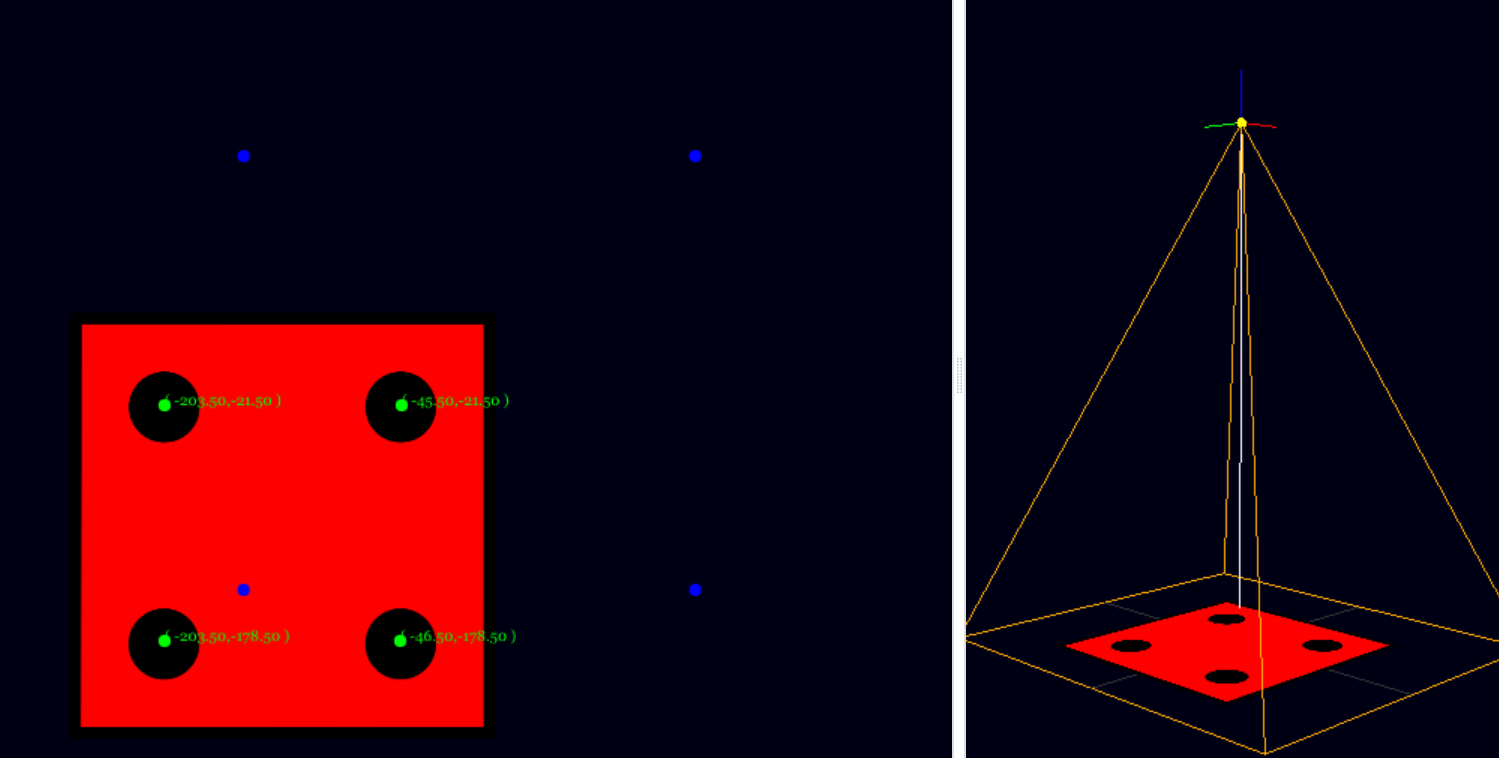
\includegraphics[width=0.8\columnwidth]{images/fig-temp1.png}
\caption{3D Servoing Environment, renderer image(left), and 3D objects(right)}
\label{fig1}
\end{center}
\end{figure}

DQN training is based on Q-learning\cite{ref1} algorithm, using Q-network for approximating Q-table. Experience replay and target Q are also applied to our method to prevent divergence and  stablize the process. For every timestep $t$, environment $\varepsilon$, composed of states$s_t$ actions $a_t$, and rewards $r_t$ are defined. The agent of DQN has Q-network $Q(s, a) -> r$, predicts rewards of each action values, so user-defined reward can backpropagate and update weight inside the network\cite{ref2}. In our proposed method, we simply set the state as four error vectors of 2D target points and corresponding ground-truth points. If the total amount of the error is decreased in $x_{t+1}$, the agent gets reward of value $1.0$, and if the error is increased, the reward is $-1.0$. The total experience size of sequence is set to $30000$, and the $a$ are consist of six actions as mentioned: forward, backward, up, down, right, left. For each actions, all the distance the camera move is $1$. The agent interacts with the simulator by selecting actions in a way that maximises future rewards. The neural network inside the agent is composed of a simple four-layered neural network composed of input layer, two fully-connected layers with 50 neurons, and regression output layer Fig. ~\ref{fig2}.

\begin{equation}\label{actions}
  a = {a_{Forward}, a_{Backward}, a_{Up}, a_{Down}, a_{Right}, a_{Left}}
\end{equation}


\tikzset{%
  every neuron/.style={
    circle,
    draw,
    minimum size=1cm
  },
  neuron missing/.style={
    draw=none,
    scale=4,
    text height=0.333cm,
    execute at begin node=\color{black}$\vdots$
  },
}
\begin{figure}[htb]
\begin{center}
  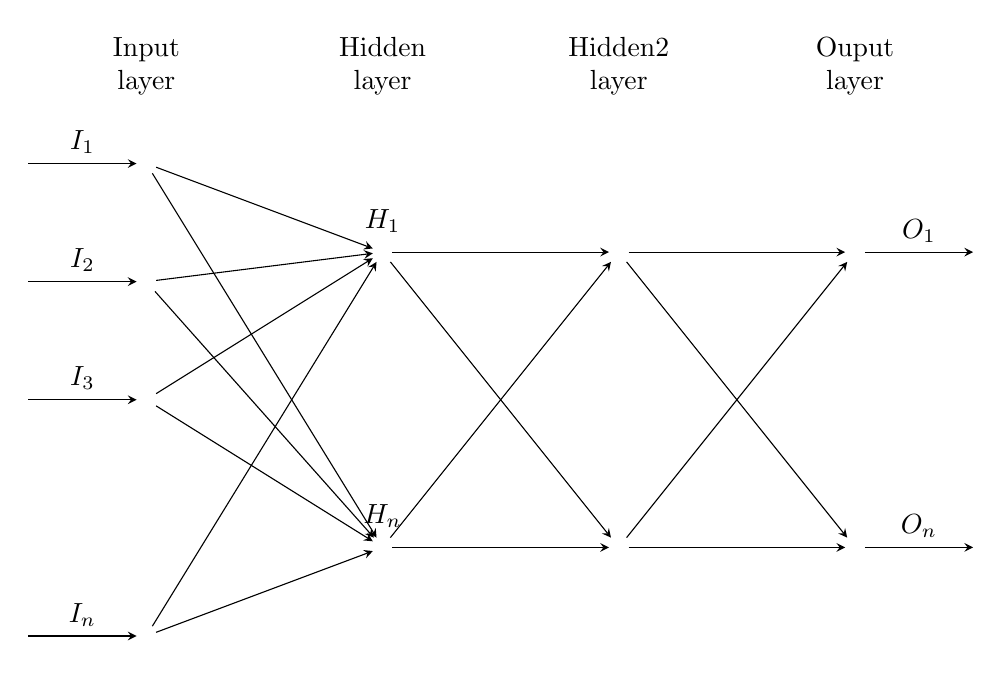
\begin{tikzpicture}[x=1.5cm, y=1.5cm, >=stealth]

  \foreach \m/\l [count=\y] in {1,2,3,missing,4}
    \node [every neuron/.try, neuron \m/.try] (input-\m) at (0,2.5-\y) {};

  \foreach \m [count=\y] in {1,missing,2}
    \node [every neuron/.try, neuron \m/.try ] (hidden-\m) at (2,2-\y*1.25) {};

  \foreach \m [count=\y] in {1,missing,2}
    \node [every neuron/.try, neuron \m/.try ] (hidden2-\m) at (4,2-\y*1.25) {};

  \foreach \m [count=\y] in {1,missing,2}
    \node [every neuron/.try, neuron \m/.try ] (output-\m) at (6,2-\y*1.25) {};

  \foreach \l [count=\i] in {1,2,3,n}
    \draw [<-] (input-\i) -- ++(-1,0)
      node [above, midway] {$I_\l$};

  \foreach \l [count=\i] in {1,n}
    \node [above] at (hidden-\i.north) {$H_\l$};

  \foreach \l [count=\i] in {1,n}
    \draw [->] (output-\i) -- ++(1,0)
      node [above, midway] {$O_\l$};

  \foreach \i in {1,...,4}
    \foreach \j in {1,...,2}
      \draw [->] (input-\i) -- (hidden-\j);

  \foreach \i in {1,...,2}
    \foreach \j in {1,...,2}
      \draw [->] (hidden-\i) -- (hidden2-\j);

  \foreach \i in {1,...,2}
    \foreach \j in {1,...,2}
      \draw [->] (hidden2-\i) -- (output-\j);

  \foreach \l [count=\x from 0] in {Input, Hidden, Hidden2, Ouput}
    \node [align=center, above] at (\x*2,2) {\l \\ layer};

  \end{tikzpicture}
\caption{Neural Network Inside the agent}
\label{fig2}
\end{center}
\end{figure}


The training process starts after first $100$ steps of random actions. Basically, the position of camera is randomly set where all four target feature points are visible. If the amount of error value of current state $x_t$ is less than $10.0$ the camera is repositioned to a random position. The agent takes input state $x_t$ and forward network, it returns a index of action that has maximum possibioity of network output. The camera carry out action which agent picked, calculate $x_{t+1}$, and reward. The agent takes reward and update the weights

 \begin{algorithm}
   \caption{DQN training process for point-based visual servoing}\label{euclid}
   \begin{algorithmic}[1]

     \State camera.RandomPosition()


     \For {$t$ in $T$}

     \State $a_t$ = brain.Forward($x_t$)
     \State camera.GoTo($a_t$)
     \State $E$ = Error($x_{t+1}$) - Error($x_t$)
     \If {E $\geq$ 0}
     \State $r_t$ = $1.0$
     \Else
     \State $r_t$ = -$1.0$
     \EndIf

     brain.Backward($r_t$)
     \If{$r_t$ $leq$ 10.0}
     camera.RandomPosition()
     \EndIf

     \EndFor

   \end{algorithmic}
 \end{algorithm}


\section{Results}
(Some Pictures)

(Graph during training)



\section{Discussion}
 Our proposed DQN model trained using each timestep's 2D feature errors, decided correct action for servoing virtual camera in 3D space. After approximately ???? steps with 64 batchs, and ?????? games with 10 batchs, the average loss and servoing time were oscillated without increasing or decreasing. From this timestep point on, we could regard that our model is well-trained and no further training is meaningless. Our well-trained model can conduct registration from a random position to the optimal position within average of ??? seconds. The visualized camera moved smoothly with almost no unnecessary movement. Compare to conventional method, such as tree searching algorithm or solving jacobi matrices, our proposed method has several benefits. First, the amount of calculation is greatly reduced. conventional method requires large amount of computations. For example, jacobi matrix calculation method needs to calculate inverse or pseudoinverse matrix in each timestep. Random searching method also requires additional calculation: feature error variation, and shows too much unnecessary movement of camera. DQN method requires such calculation only when it is being trained. Once training task is done, this does not require complex computation, and shows efficient servoing movement.

 For now, there are several limitations that need to be improved. First, the camera movement has restrictions compare to the jacobi matrix method. The jacobi matrix calculation method results all-round 3D translation and rotation vector; In our current condition, the movement could only be one of six normalized direction vectors, and no rotations. Under this condition the camera movements looks a little awkward showing staircase. Since all the distance the camera move is $1$, it is also inefficient in terms of utilization of error sizes. Second, states $x_t$ is too simple to apply to 2D-3D registrations. Our current method defined $x_t$ as four 2D point vector errors, but real 2D-3D registration, larger and much more complex features need to be used to define current state.

 Those limitations can be possibly resolved in the future works. As for the camera movement problem, adding rotation action and combining camera action according to the whole output matrix of Q-network can solve most of its problems.


But in the future, this can possibily be overcome.
firstly, camera movement can be simply more natural and sophisticated, by using the whole network output and possibilities.
Rotation can be also added and perform similarily.

secondly, Input state can be defined by using whole rendered image of camera. There are lot of image-handling deep neural networks proposed, we can simply replace our network to one of them.



\section{Conclusion}

We have developed visual servoing simulator using deep Q learning method.

Although there are several limitations for now, there are possible future work can overcome them.

Our visual servoing simulator takes 2D feature point vector errors, and decide camera how to move in 3D space.

This future work can be integrated in near future, and this can perform as 2D-3D registration simulator


\section*{Acknowledgement}
This research was supported by the KIST institutional program (??????, ???????).


\bibliographystyle{elsarticle-num}
\bibliography{references}

%
% \begin{thebibliography}{9}
% \bibitem{ref1}
% S.~Fortune, A sweepline algorithm for Voronoi diagrams,
% {\it Algorithmica} {\bf 2} (1987), pp.153--174.
%
% \bibitem{ref2}
% G.~Farin, {\it Curves and Surfaces for Computer Aided Geometric
% Design: A Practical Guide}, Academic Press, San Diego, 1988.
%
% \bibitem{ref3}
% A. Okabe, B. Boots, K. Sugihara, and S.N. Chiu,
% {\it Spatial Tessellations: Concepts and Applications of
% Voronoi Diagrams}, 2nd Edition, John Wiles \& Sons, Chichester, 2000.
%
% \bibitem{ref4}
% T. Pavlidis, Curve fitting with conic splines,
% {\it ACM Transactions on Graphics} {\bf 19} (1983), pp. 151--159.
%
% \bibitem{ref5}
% K. Sugihara's Homepage,
% \texttt{http://www.simplex.t.u-tokyo.ac.jp/\~{}sugihara/}, 2005.
%
% \bibitem{ref6}
% G. Taubin, A signal processing approach to fair surface design,
% in {\it Proc. of SIGGRAPH} (1995), pp. 351--358.
%
% \end{thebibliography}

\end{document}
